\documentclass[11pt,a4paper,]{article}
\usepackage{lmodern}
\usepackage{amssymb,amsmath}
\usepackage{ifxetex,ifluatex}
\usepackage{fixltx2e} % provides \textsubscript
\ifnum 0\ifxetex 1\fi\ifluatex 1\fi=0 % if pdftex
  \usepackage[T1]{fontenc}
  \usepackage[utf8]{inputenc}
\else % if luatex or xelatex
  \ifxetex
    \usepackage{mathspec}
  \else
    \usepackage{fontspec}
  \fi
  \defaultfontfeatures{Ligatures=TeX,Scale=MatchLowercase}
\fi
% use upquote if available, for straight quotes in verbatim environments
\IfFileExists{upquote.sty}{\usepackage{upquote}}{}
% use microtype if available
\IfFileExists{microtype.sty}{%
\usepackage{microtype}
\UseMicrotypeSet[protrusion]{basicmath} % disable protrusion for tt fonts
}{}
\usepackage[margin=1in]{geometry}
\usepackage{hyperref}
\hypersetup{unicode=true,
            pdftitle={Who we are affects how we vote},
            pdfauthor={Rob J Hyndman and Di Cook},
            pdfborder={0 0 0},
            breaklinks=true}
\urlstyle{same}  % don't use monospace font for urls
\usepackage[style=authoryear-comp]{biblatex}

\addbibresource{references.bib}
\usepackage{longtable,booktabs}
\usepackage{graphicx,grffile}
\makeatletter
\def\maxwidth{\ifdim\Gin@nat@width>\linewidth\linewidth\else\Gin@nat@width\fi}
\def\maxheight{\ifdim\Gin@nat@height>\textheight\textheight\else\Gin@nat@height\fi}
\makeatother
% Scale images if necessary, so that they will not overflow the page
% margins by default, and it is still possible to overwrite the defaults
% using explicit options in \includegraphics[width, height, ...]{}
\setkeys{Gin}{width=\maxwidth,height=\maxheight,keepaspectratio}
\IfFileExists{parskip.sty}{%
\usepackage{parskip}
}{% else
\setlength{\parindent}{0pt}
\setlength{\parskip}{6pt plus 2pt minus 1pt}
}
\setlength{\emergencystretch}{3em}  % prevent overfull lines
\providecommand{\tightlist}{%
  \setlength{\itemsep}{0pt}\setlength{\parskip}{0pt}}
\setcounter{secnumdepth}{5}
% Redefines (sub)paragraphs to behave more like sections
\ifx\paragraph\undefined\else
\let\oldparagraph\paragraph
\renewcommand{\paragraph}[1]{\oldparagraph{#1}\mbox{}}
\fi
\ifx\subparagraph\undefined\else
\let\oldsubparagraph\subparagraph
\renewcommand{\subparagraph}[1]{\oldsubparagraph{#1}\mbox{}}
\fi

%%% Use protect on footnotes to avoid problems with footnotes in titles
\let\rmarkdownfootnote\footnote%
\def\footnote{\protect\rmarkdownfootnote}

%%% Change title format to be more compact
\usepackage{titling}

% Create subtitle command for use in maketitle
\providecommand{\subtitle}[1]{
  \posttitle{
    \begin{center}\large#1\end{center}
    }
}

\setlength{\droptitle}{-2em}

  \title{Who we are affects how we vote}
    \pretitle{\vspace{\droptitle}\centering\huge}
  \posttitle{\par}
    \author{Rob J Hyndman and Di Cook}
    \preauthor{\centering\large\emph}
  \postauthor{\par}
    \date{}
    \predate{}\postdate{}
  
%% Any special functions or other packages can be loaded here.

\usepackage[no-weekday]{eukdate}
\usepackage{sourceserifpro}
\usepackage[scaled=0.86]{DejaVuSansMono}
\usepackage{float,bm,setspace}
\setstretch{1.2}

%% CAPTIONS
\RequirePackage{caption}
\DeclareCaptionStyle{italic}[justification=centering]
 {labelfont={bf},textfont={it},labelsep=colon}
\captionsetup[figure]{style=italic,format=hang,singlelinecheck=true}
\captionsetup[table]{style=italic,format=hang,singlelinecheck=true}

%% GRAPHICS
\RequirePackage{graphicx}
\setcounter{topnumber}{2}
\setcounter{bottomnumber}{2}
\setcounter{totalnumber}{4}
\renewcommand{\topfraction}{0.85}
\renewcommand{\bottomfraction}{0.85}
\renewcommand{\textfraction}{0.15}
\renewcommand{\floatpagefraction}{0.8}

%% BIBLIOGRAPHY

\makeatletter
\@ifpackageloaded{biblatex}{}{\usepackage[style=authoryear-comp, backend=biber, natbib=true]{biblatex}}
\makeatother
\ExecuteBibliographyOptions{bibencoding=utf8,minnames=1,maxnames=3, maxbibnames=99,dashed=false,terseinits=true,giveninits=true,uniquename=false,uniquelist=false,doi=false, isbn=false,url=true,sortcites=false}

\DeclareFieldFormat{url}{\texttt{\url{#1}}}
\DeclareFieldFormat[article]{pages}{#1}
\DeclareFieldFormat[inproceedings]{pages}{\lowercase{pp.}#1}
\DeclareFieldFormat[incollection]{pages}{\lowercase{pp.}#1}
\DeclareFieldFormat[article]{volume}{\mkbibbold{#1}}
\DeclareFieldFormat[article]{number}{\mkbibparens{#1}}
\DeclareFieldFormat[article]{title}{\MakeCapital{#1}}
\DeclareFieldFormat[inproceedings]{title}{#1}
\DeclareFieldFormat{shorthandwidth}{#1}
% No dot before number of articles
\usepackage{xpatch}
\xpatchbibmacro{volume+number+eid}{\setunit*{\adddot}}{}{}{}
% Remove In: for an article.
\renewbibmacro{in:}{%
  \ifentrytype{article}{}{%
  \printtext{\bibstring{in}\intitlepunct}}}

\makeatletter
\DeclareDelimFormat[cbx@textcite]{nameyeardelim}{\addspace}
\makeatother
\renewcommand*{\finalnamedelim}{%
  %\ifnumgreater{\value{liststop}}{2}{\finalandcomma}{}% there really should be no funny Oxford comma business here
  \addspace\&\space}

\begin{document}
\maketitle

\hypertarget{intro}{%
\section{Introduction}\label{intro}}

We often hear commentary about voting patterns --- people in their 20s without kids are more likely to be left wing, migrants are more conservative, wealthier people tend to favour the conservative parties, and so on. These might be built on myth and stereotypes. There is open data available from each election and from regular national censuses; this data can be used to examine just what are the indicators for voting tendency.

Voting tendencies can change over time. For example, if wealth was a good predictor of conservative voting in the 2001 election, is it still a good predictor in 2019? Australia has changed in many ways over the last two decades. Rising house prices, country-wide improvements in education, an ageing population, and a decline in religious affiliation, are just some of the ways we have changed. At the same time, political power has moved back and forth between the two major parties. How much can we attribute changes in political power to changes in who we are?

\hypertarget{census-and-electoral-data}{%
\section{Census and electoral data}\label{census-and-electoral-data}}

The Census provides data on electoral socio-demographics, and vote counts in each electorate can be obtained from Australian federal elections. However, joining these two data sources is difficult because the Censuses are not held at the same time as the elections. Between 2001 and 2016 there were six elections and four Censuses, as shown in the timeline below.

\begin{figure}[H]

{\centering 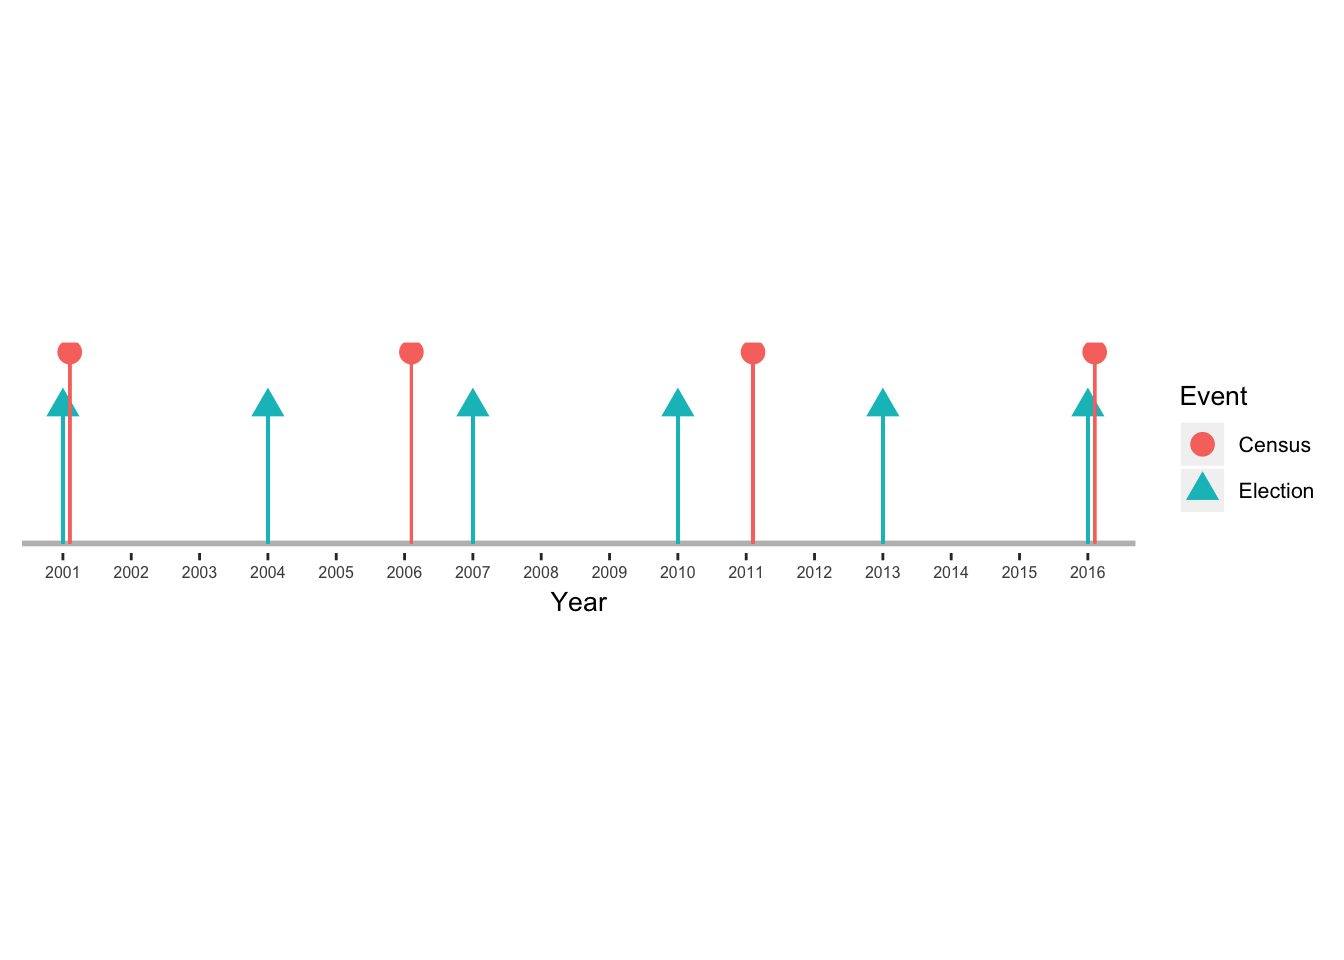
\includegraphics{elections_conversation_files/figure-latex/timeline-1} 

}

\caption{Timeline of Australian elections and Censuses. Censuses happen regularly, elections not quite regularly, which means data needs to be interpolated by time.}\label{fig:timeline}
\end{figure}

Not only can an electorate change between the last Census and an election, but even the electorate boundaries can change. Some electorates can disappear altogether and new electorates can arise. Electoral boundaries are redistributed regularly by the AEC, meaning that only in the years where both a Census and an election occur are all boundaries likely to match --- the case for the 2001 and 2016 elections. So we first had to estimate what the socio-demographic characteristics of an electorate would have been at the time of each election using a complicated method of interpolation over time and geography. This method uses Census information from both before and after the election of interest, and information from neighbouring electorates when boundaries have changed.

\hypertarget{modelling}{%
\section{2PP Modelling}\label{modelling}}

A simple way to measure voting patterns is to consider the two-party preferred (2PP) vote, which is based on the tally of preferences for the Labor and Liberal candidates, ignoring all other candidates. By convention, this is recorded as a percentage preference in favour of the Liberal party --- for example, a 2PP value of 45\% indicates that 45\% of voters ranked the Liberal candidate higher than the Labor candidate, while the remaining 55\% ranked them in the reverse order.

We consider how various socio-demographic variables obtained from Census data can be used to explain the 2PP values for each of the 150 electorates in each of the federal elections between 2001 and 2016.

Many of the socio-demographic variables have changing scales over the years. For example, inflation-adjusted median rental prices increased across almost all electorates, with median rent of 200 dollars per week placing an electorate in the 90th percentile in 2001, but only the 30th percentile in 2016. In order for socio-demographic effects to be comparable across years, all socio-demographic variables were standardized.

There are dozens of socio-demographic variables available in the Censuses, with many variables representing similar information about an electorate. So we combined some variables to avoid redundant information. For example, our ``Incomes'' variable is a combination of median personal income, household income and family income.

We are using data at the electorate level. The results do not directly address the voting intentions of individuals.

Each election was modelled separately, to allow us to see any changes over time, and to account for changing electorate boundaries. In this article, we highlight the variables with the strongest relationship to the two-party preferred vote, or which have had substantial changes over time. The full analysis is available at \url{https://robjhyndman.com/publications/elections/}.

\hypertarget{country-wide-trend}{%
\subsection*{Country-wide trend}\label{country-wide-trend}}
\addcontentsline{toc}{subsection}{Country-wide trend}

First, we show the estimated two-party preferred vote for an ``average'' electorate.

\begin{figure}[H]

{\centering 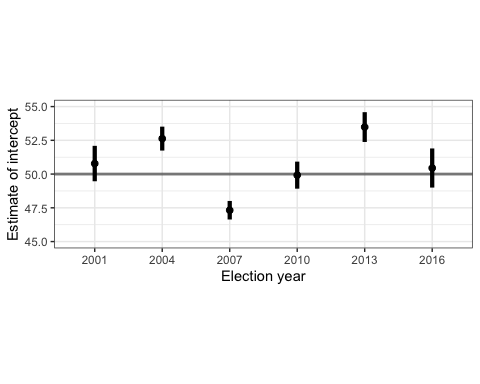
\includegraphics{elections_conversation_files/figure-latex/plotintercept-1} 

}

\caption{Estimated two-party preferred vote for an electorate with average characteristics at each election.}\label{fig:plotintercept}
\end{figure}

This shows that the baseline of party preference has varied over the elections, with the biggest swing occurring in the 2007 election where the mean electorate shifted more than five percentage points in favour of the Labor party. The dots represent the estimated 2PP value, and the lines indicate a 95\% confidence interval providing a guide to the uncertainty in the estimate. Where the vertical lines corresponding to each election cross the 50\% horizontal line, the 2PP vote for an average electorate is not statistically distinguishable from 50\% for that election.

\hypertarget{age}{%
\subsection*{Age}\label{age}}
\addcontentsline{toc}{subsection}{Age}

Regions comprising more older people are often believed to be more conservative, and indeed we found that electorates with a higher median age are more likely to support the Liberal party --- although this effect is significant only in 2004 and 2007.

\begin{figure}[H]

{\centering \includegraphics{elections_conversation_files/figure-latex/age-1} 

}

\caption{Estimated impact of electorate median age on the two-party preferred vote.}\label{fig:age}
\end{figure}

This graph shows the effect of median age on the 2PP vote. The vertical scale can be interpreted as a score measuring how much the 2PP vote differs between an average electorate, and an electorate with median age in the top 10\% of all electorates (with all other socio-demographic variables unchanged). The reverse is true for young electorates --- the score can be interpreted as how much the 2PP vote would be reduced if an average electorate kept all socio-demographic variables fixed but median age was reduced to be in the bottom 10\% of all eletorates.

\hypertarget{income}{%
\subsection*{Income}\label{income}}
\addcontentsline{toc}{subsection}{Income}

Typically the Labor party campaigns on more progressive policies, which often include tax reform that adversely affects higher income earners, and more generous social assistance programs. Perhaps it is due to these policies that higher income electorates appear more likely to support the Liberal party, as the \texttt{Incomes} factor has a positive effect on Liberal preference. The effect also seems to have been increasing over time.

\begin{figure}[H]

{\centering \includegraphics{elections_conversation_files/figure-latex/income-1} 

}

\caption{Estimated impact of electorate income on the two-party preferred vote.}\label{fig:income}
\end{figure}

As before, the vertical scale can be interpreted as a score measuring how much the 2PP vote differs between an average electorate, and an electorate with income in the top 10\% of all electorates (with all other socio-demographic variables unchanged).

\hypertarget{unemployment}{%
\subsection*{Unemployment}\label{unemployment}}
\addcontentsline{toc}{subsection}{Unemployment}

Unemployment however, is not as influential. In 2001 and 2004, electorates with higher unemployment align with Labor, but over time this shifts towards support for the Liberal party, culminating in a significantly positive (but small) effect in 2016.

\begin{figure}[H]

{\centering \includegraphics{elections_conversation_files/figure-latex/unemployment-1} 

}

\caption{Estimated impact of electorate unemployment on the two-party preferred vote.}\label{fig:unemployment}
\end{figure}

The vertical scale can be interpreted as a score measuring how much the 2PP vote differs between an average electorate, and an electorate with unemployment in the top 10\% of all electorates (with all other socio-demographic variables unchanged)

\hypertarget{industry-and-type-of-work}{%
\subsection*{Industry and type of work}\label{industry-and-type-of-work}}
\addcontentsline{toc}{subsection}{Industry and type of work}

Electorates with higher proportions of workers in extractive industries (mining, gas, water, agriculture, waste and electricity) are consistently linked with higher support for the Liberal party, with the magnitude of this effect slightly increasing over the years.

\begin{figure}[H]

{\centering \includegraphics{elections_conversation_files/figure-latex/extractive-1} 

}

\caption{Estimated impact of employment in the extractive industries on the two-party preferred vote.}\label{fig:extractive}
\end{figure}

This is unsurprising, as the Liberal party has close ties with these traditional energy industries, and typically present policies to reduce taxation on energy production.

Electorates with more workers in transformative industries (construction or manufacturing) are also more likely to support the Liberal party.

\begin{figure}[H]

{\centering \includegraphics{elections_conversation_files/figure-latex/transformative-1} 

}

\caption{Estimated impact of employment in the transformative industries on the two-party preferred vote.}\label{fig:transformative}
\end{figure}

The proportion of workers in managerial, administrative, clerical and sales roles is also a significant predictor of two-party preference vote across all six elections, with a higher proportion of people working these jobs increasing Liberal support.

\begin{figure}[H]

{\centering \includegraphics{elections_conversation_files/figure-latex/manager-1} 

}

\caption{Estimated impact of employment in management or administration on the two-party preferred vote.}\label{fig:manager}
\end{figure}

\hypertarget{household-mobility}{%
\subsection*{Household mobility}\label{household-mobility}}
\addcontentsline{toc}{subsection}{Household mobility}

In each of the six elections, electorates with a higher proportion of people that have recently (in the past five years) moved house are more likely to support the Liberal party.

\begin{figure}[H]

{\centering \includegraphics{elections_conversation_files/figure-latex/mobility-1} 

}

\caption{Estimated impact of household mobility on the two-party preferred vote.}\label{fig:mobility}
\end{figure}

Our analysis controls for characteristics of home ownership and rental prices, so this effect is not simply due to electorates having low rates of home ownership, or due to electorates having high rental prices. Instead, it suggests that people who are more transient are also more likely to be conservative voters, regardless of their home ownership or rental status. (This would need further study, as we do not have individual level voting data.)

\hypertarget{relationships}{%
\subsection*{Relationships}\label{relationships}}
\addcontentsline{toc}{subsection}{Relationships}

De facto relationships, but not marriages, are found to be an important (and significant) predictor of the two-party preferred vote in all six elections, with more de facto relationships associated with higher support for the Labor party. The proportion of individuals who are married however, is insignificant (not shown).

\begin{figure}[H]

{\centering \includegraphics{elections_conversation_files/figure-latex/defacto-1} 

}

\caption{Estimated impact of de facto relationships on the two-party preferred vote.}\label{fig:defacto}
\end{figure}

\hypertarget{education}{%
\subsection*{Education}\label{education}}
\addcontentsline{toc}{subsection}{Education}

Since 2007, electorates with higher education levels are associated with supporting the Labor party, although this effect is significant only in 2016. Before 2007, education had a negligible effect.

\begin{figure}[H]

{\centering \includegraphics{elections_conversation_files/figure-latex/education-1} 

}

\caption{Estimated impact of education on the two-party preferred vote.}\label{fig:education}
\end{figure}

\hypertarget{diversity}{%
\subsection*{Diversity}\label{diversity}}
\addcontentsline{toc}{subsection}{Diversity}

Larger migrant populations from Asia, the Middle East, South-Eastern Europe, the United Kingdom and elsewhere, are either associated with Labor support, or have no effect. Of these areas, only differences in South-Eastern European populations appear to have had a significant impact in each election, with the proportion of Asian migrants also being significant in 2010.

Speaking languages other than English however, appears to have a far stronger effect. Electorates with more diverse languages are associated with higher support for the Liberal party from 2004 onwards, with this effect being significant in 2007, 2010 and 2016.

\begin{figure}[H]

{\centering \includegraphics{elections_conversation_files/figure-latex/otherlanguage-1} 

}

\caption{Estimated impact of ethnic diversity on the two-party preferred vote.}\label{fig:otherlanguage}
\end{figure}

Of the variables relating to religion, only Judaism shows a consistent effect, with electorates with relatively large Jewish populations more likely to vote Liberal.

\hypertarget{state-effects}{%
\section{State effects}\label{state-effects}}

It is often suggested that states have systematic differences that cause their electorates to vote differently. We can explore this effect by looking at the difference between the actual 2PP vote in each electorate and what our modelling would predict based only on electorate characteristics. We found a bias toward Labor in the ACT, and to a smaller extent in Tasmania, and a bias toward the Liberals in the Northern Territory. No other states showed a significantly different voting pattern from what you would expect using only socio-demographic information. That suggests that any differences between Queensland and Victoria (for example) are due to different voter socio-demographics.

\hypertarget{against-the-tide}{%
\section{Against the tide}\label{against-the-tide}}

As well as looking at whether some states have results different from what is predicted, we can also look at individual electorates. That is, when does an electorate vote very differently from what their socio-demographics would suggest? This suggests something is going on beyond the effect of socio-demographics. For example, a very good (or bad) local member could lead to voting patterns that are very different from what is predicted.

Based on the distribution of the Cook's distance values, a Cook's distance greater than \(0.1\) is considered to be influential and a potential outlier. The electorate of Sydney (NSW) has a large Cook's distance from 2001 to 2013, due to its diverse population (language, birthplace and religion), high number of defacto relationships, high income, high household mobility and small amount of workers in extractive and transformative jobs. It has remained a strong supporter of the Labor party and the Liberal vote is severely overpredicted by the model, making it an outlier. Nearby in metropolitan NSW, the electorate of Wentworth is found to be an outlier in all but the 2007 election. Although historically Liberal, its two-party vote jumped by over 10 percentage points in 2010 without experiencing any notable changes in its socio-demographic makeup --- implying that this may be the direct effect of its Liberal member, Malcolm Turnbull, becoming the leader of the Liberal party. Liberal support in Wentworth is underpredicted by the model in each year, and more so with Turnbull as Liberal leader.

Lingiari, an electorate taking up almost all of the Northern Territory, is an outlier in the 2001--2007 elections due to its large Indigenous population, young age profile and low rates of property ownership. Fowler (NSW) has a diverse population with a high proportion of migrants, many Buddhists and Muslims, and has strong Labor support, making it influential in 2001, 2004 and 2010. Other electorates with large Cook's distance are Barton (NSW) and Leichhardt (QLD) in 2016, and Canberra (ACT) in 2007.

\hypertarget{conclusion}{%
\section{Conclusion}\label{conclusion}}

This paper explores the effects of electoral socio-demographic characteristics on the two-party preferred vote in the 2001--2016 elections, using information from the corresponding Australian federal elections and Censuses. As a Census does not always occur in the same year as an election, Census data for the 2004--2013 elections are generated by employing a method of spatio-temporal imputation. This imputes electoral socio-demographics for the electoral boundaries in place at the time of the election --- an approach that is distinctly different from previous work on modelling election outcomes, where Census and election data are typically joined without addressing their temporal differences. Before estimating a model, these socio-demographic variables are standardized (to adjust for changing variable scales) and many variables (representing similar information) are combined into factors, resulting in a reduced predictor set. A spatial error model is then estimated for each election, accounting for the inherent spatial structure of the data.

Across the past six elections, most of the socio-demographics that drive the electoral two-party preferred vote are found to remain steady, whilst a few (typically weaker) effects vary over time. Industry and type of work are particularly influential, with energy-related and manufacturing/construction jobs, as well as administrative roles being strongly linked with the Liberal party in all elections. Incomes have a similarly consistent effect, with higher income areas supporting Liberal. Higher levels of unemployment shift from weak association with Labor to a significant Liberal effect over the years, and higher education levels are associated with Labor from 2007 (although significant only in 2016). It is also found that electorates with higher household mobility support Liberal, birthplace diversity favours Labor and more de facto relationships align with Labor preference --- although marriages, family and household sizes have no material influence. Furthermore, the neighbourhood (spatial) effects are found to be positive in all elections, although significant only in 2001 and 2016, meaning that in the 2004--2013 elections, electorates effectively voted independently.

The findings in this paper complement the existing literature by modelling temporal trends, which as far as the authors are aware, has not been done previously for Australian elections using a regression framework. It is also the first study to model any Australian election since 2010 using Census information.

Additionally, a key contribution of this research is the wrangling of the raw data and imputed data sets for the 2004, 2007, 2010 and 2013 elections, which have been contributed to the \texttt{eechidna} \texttt{R} package --- providing a rich, accessible data resource for future Australian electoral analysis.

\hypertarget{acknowledgements}{%
\section{Acknowledgements}\label{acknowledgements}}

This paper was produced using \texttt{RMarkdown} \autocite{rmarkdown} and \texttt{knitr} \autocite{knitr}. All corresponding code for this paper can be found in the github repository \href{https://github.com/jforbes14/eechidna-paper}{github.com/jforbes14/eechidna-paper}, and the data used is available in the \texttt{eechidna} package \autocite{eechidna}. All raw data was obtained from the Australian Electoral Commission, the Australian Bureau of Statistics and the Australian Government.

\hypertarget{software}{%
\section{Software}\label{software}}

All election and Census datasets, along with electoral maps and more, are available in the \texttt{eechidna} (Exploring Election and Census Highly Informative Data Nationally for Australia) \texttt{R} package, which can be downloaded from CRAN. The \texttt{eechidna} package makes it easy to look at the data from the Australian Federal elections and Censuses that occurred between 2001 and 2016. This study contributed a large revision to the \texttt{eechidna} package, which included the addition of election and Census data for 2001--2010, voting outcomes for polling booths and imputed Census data for election years. For more details on using \texttt{eechidna}, please see the articles (vignettes) on the github page \href{https://ropenscilabs.github.io/eechidna/}{ropenscilabs.github.io/eechidna/}.

The authors would like to sincerely thank Anthony Ebert, Heike Hofmann, Thomas Lumley, Ben Marwick, Carson Sievert, Mingzhu Sun, Dilini Talagala, Nicholas Tierney, Nathaniel Tomasetti, Earo Wang and Fang Zhou, all of whom have contributed to the \texttt{eechidna} package.

\printbibliography


\end{document}
